\section{Implementation}\label{ms:sec:expe}
In this section, we discuss the realization of our approach for its practical deployment. The components that have to be considered are the {\em client\/}, who decrypts resources to access them (Section~\ref{ms:sec:client}), and the {\em protocol\/} used for the interaction between client and server. The protocol has a significant impact on the profile of the {\em server\/} responsible for hosting the resources and for authenticating the data owner who is the only party authorized to modify the data. In particular, we will consider two options for the realization of the interaction protocol: {\em i) Overlay\/} (Section~\ref{ms:sec:overlay}), which operates on top of a common cloud object service (the server is unaware of the adoption of our approach and is a standard object server); and {\em ii) Ad-hoc} (Section~\ref{ms:sec:adhoc}), which directly supports the primitives to update a fragment and to get the current state of the resource (the server is aware of the features of our approach and attention will have to be paid to its internal structure).
 
We found from this analysis that the client is able to make use of our approach without restrictions, with a performance in the application of the technique for a common personal computer that does not represent a bottleneck when compared with any network bandwidth. For the protocol, when the technique is applied in a transparent way on top of existing object storage solutions (Overlay), we observe several orders of magnitude in performance improvement for some configurations. The realization of the technique using an ad-hoc protocol further improves the benefits with its greater flexibility, but it also requires to consider the mapping of the logical structure to its physical representation - for which we have identified an adequate solution. All these results prove the applicability of the technique in the current technological landscape and the benefits that it can provide for many application domains.

It is important to observe that the primary parameters influencing the performance are the size \msize\ of mini-block and the number \fnum\ \! of fragments. While the size of mini-blocks represents our security parameter and must be chosen by the data owner based on her security requirements, the number of fragments is chosen considering performance only. In the following, we will then focus on the tuning of the number of fragments, considering resources of variable sizes. (Note that the choice of the number of fragments implies also the definition of the number of macro-blocks, as the product of the number of macro-blocks by the number of fragments is equal to the number of mini-blocks of the resource.)

The evaluation of the best value for the number of fragments will have to consider a number of aspects that characterize the application domain. The major ones are: frequency of policy updates; frequency and average size of {\tt get} requests; network bandwidth, for the upload and download direction. All these aspects have a direct impact on the overall throughput offered by our solution, which confirms its advantage in the prompt enforcement of revoke operations, measured by the average transfer rate for {\tt get} requests. 

The experimental results illustrated in this section have been obtained using, for the client, a machine with Linux Ubuntu 16.04 LTS, Intel i7-4770K, 3.50 GHz, 4 cores. For the server, we used an Amazon EC2 m4.large instance, with 4 CPUs and 8 GB of RAM. The client was connected to the Internet by a symmetric 100 Mbps connection.

\subsection{Client}\label{ms:sec:client}
Our approach requires the client to execute a more complex decryption compared to the use of AES with a traditional encryption mode (e.g., CTR or CBC). The cost of decryption (which is comparable to the cost of encryption by the data owner) is nearly $\log_{\mnumb} (\mnumb \cdot \bnum)$ times the cost of applying a single AES decryption, while the impact of reorganizing the data structure at each round is limited. Due to the high performance of modern processors in the execution of block ciphers, this logarithmic cost factor is not critical. Also, decryption can be parallelized on multi-core CPUs, making the client processing even more efficient.

An aspect that has to be considered in the implementation of the client is the possible need to keep large amounts of data in memory. This may occur when fragments are downloaded one after the other and decryption can start only after the last fragment has been downloaded, which, for example, happens with the Overlay solution. If the resource size exceeds the available memory at the client, this leads to an extremely significant performance hit. The configuration of the system can (and should) avoid this possibility by splitting the resource into sub-resources (Section~\ref{ms:sec:overlay}).

\subsubsection{Experiments on the client}
\label{ms:sect:experiments}

\begin{figure}
\centering
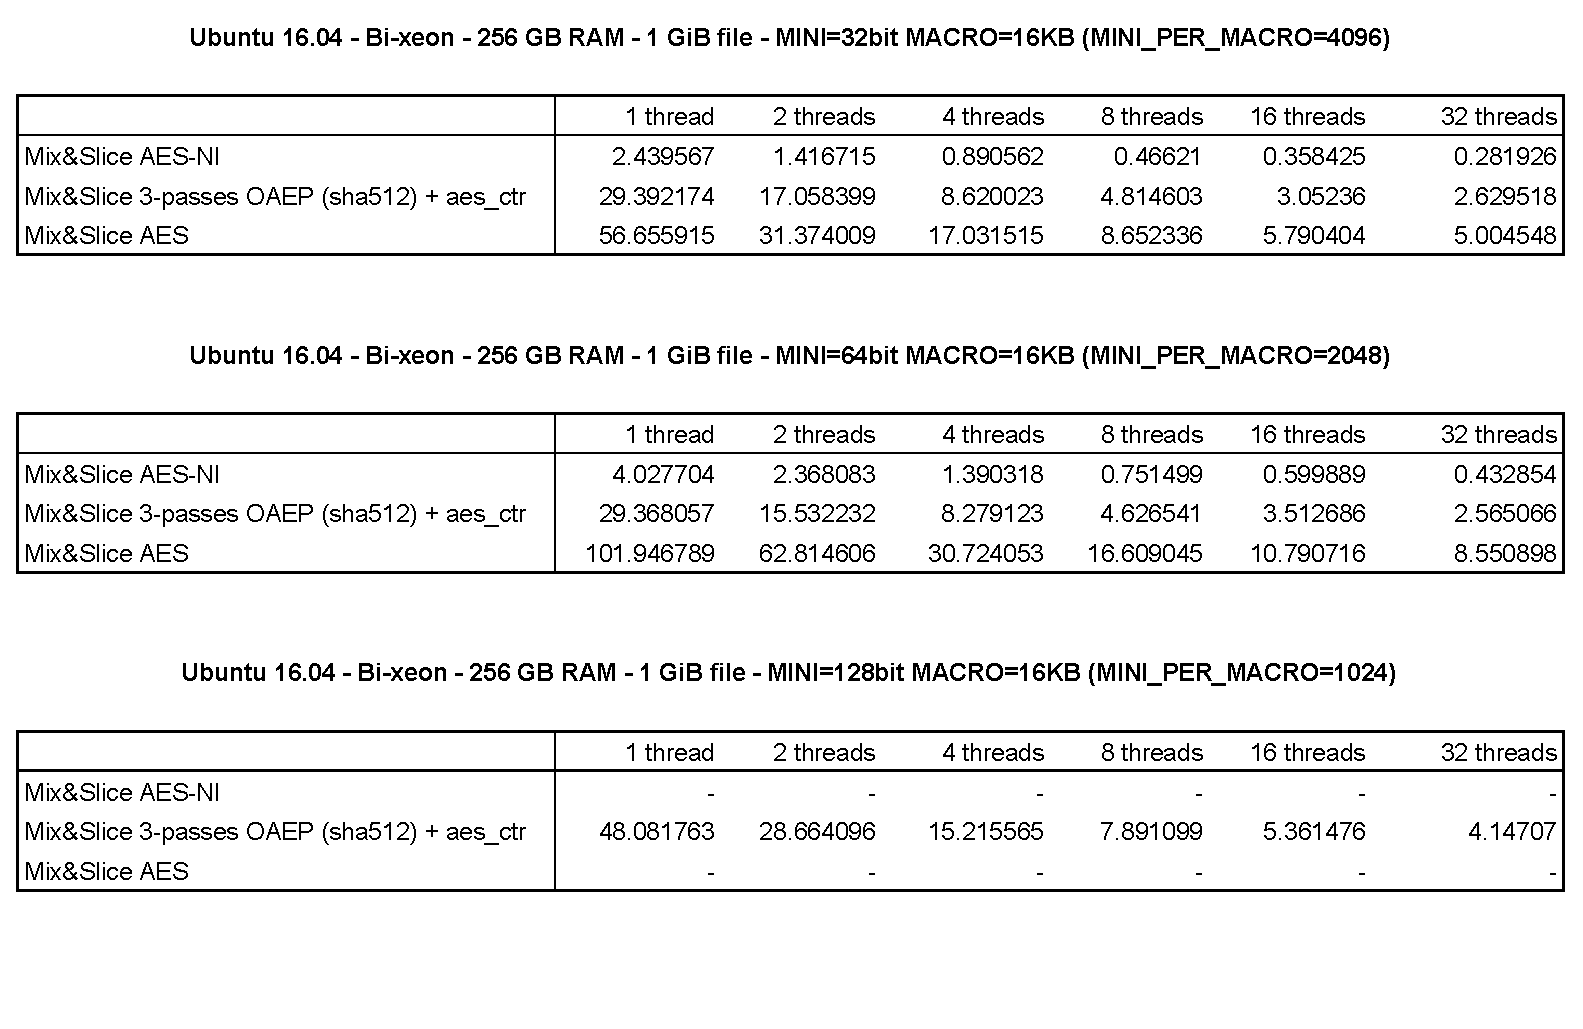
\includegraphics[width=\columnwidth,valign=t]{figures/oaep}
\caption{\label{ms:table:oaep}Performance comparison of mixing implementations}
\end{figure}

All code has been written in Python, because for all the functions the computational performance is not a constraint. The only component written in C was the invocation of the mixing for encryption and decryption functions. Since most current Intel x86 CPUs offer the support for a hardware implementation of AES, named AES-NI, we considered its adoption in our experiments. 

\new{

We implemented both the mixing structure based on AES (described in Section~\ref{ms:sect:mixing}) and the OAEP-based one (described in Section~\ref{ms:sect:oaep}) to compare their performance profile. The results are presented in Figure~\ref{ms:table:oaep}.
From the table File size, macro-block size, and mini-block size being the same, the OAEP-based implementation is faster compared to the AES one that does not leverage the hardware implementation. In fact, even tough the base application of {\em AES-128} and {\em sha-512} share a similar performance profile, the OAEP approach has a benefit due to the reduction on the number of rounds. However, on architectures that provide a native hardware implementation for {\em AES}, its use shows the best performance profile for \name and should be preferred.
As also discussed in Section~\ref{ms:sect:oaep}, the AES implementation has a maximum mini-block size of $64$ bits, whereas the OAEP implementation has a maximum mini-block size of $256$ bits. This is the reason why the third test in Figure~\ref{ms:table:oaep} shows the results of the sole OAEP implementation.

} % end \new

Figure~\ref{ms:fig:clientPerf} shows that the cost of decryption is compatible with all reasonable scenarios for the application of our technique. In particular, the figure illustrates the throughput obtained, varying the number of threads, by the application of our approach in different configurations characterized by macro-blocks of size (\Msize) 4 KiB, mini-blocks of size (\msize) 32 and 64 bits (which imply 5 and 9 encryption rounds, resp.), when using AES-NI and when not using it (AES). Mixing was applied on data that were already available in memory. We notice that even the single-threaded 9-round non-hardware-supported implementation (line `AES, \msize=64, \Msize=4096') offers a throughput that is greater than 100 Mbps. For the AES-NI multi-threaded 5-round implementation we reach a 2.5 GB/s throughput (line `AES-NI, \msize=32, \Msize=4096'). The figure also shows that, increasing the number of threads, we reach a performance level that is 4 times the one obtained by the single-threaded implementation. This is consistent with the presence of 4 physical cores in the CPU we used, each with a dedicated AES-NI circuitry.

\begin{figure}
	\centering
	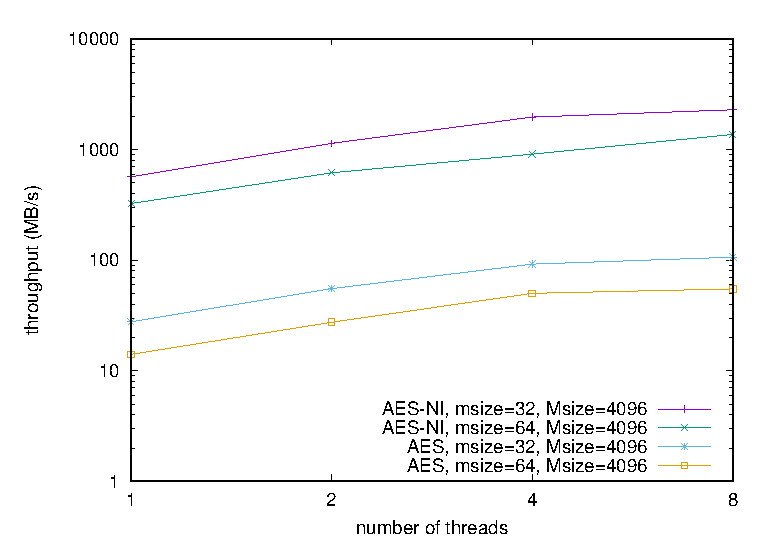
\includegraphics[width=0.8\columnwidth,valign=t]{figures/fig09}
	\caption{\label{ms:fig:clientPerf}Throughput varying the number of threads}
\end{figure}

The performance, even for a large number of fragments, shows to be orders of magnitude better than the bandwidth of current network connections. Even without the hardware support (lines `AES, \msize=32, \Msize=4096' and `AES, \msize= 64, \Msize=4096'), the application of the cryptographic transformation shows greater throughput than the data transfer rate of most Internet connections. An experiment on 1 GiB size macro-blocks and 32 bit mini-blocks showed the expected slow down in throughput, managing the decryption in less than 5 seconds (still above the bandwidth of long-distance connections).


\subsection{Overlay solution \label{ms:sec:overlay}}
The Overlay solution is analyzed using as a reference the Swift service. Swift has been selected due to its popularity, availability as open source, and technical features that are good representatives of what is offered by a modern object storage service for the cloud (resources are called {\em objects} in this discussion, to align with the Swift terminology). The Swift server instance has been installed on the Amazon EC2 platform. We consider two main alternatives for the realization of our approach on Swift\footnote{\ Swift organizes objects within {\em containers}. The current structure of Swift supports access control only at the level of containers. The analysis we present can be immediately adapted to the management of the access policy at the container granularity rather than the object granularity. We keep the analysis at the level of object for consistency with the chapter.} without any changes to the server.\footnote{\ We changed the server to support a large number of fragments in DLO mode.} The first option assumes to manage each fragment as a separate object. The second option makes use of the ability to access portions of objects and specifically considers the use of {\em Dynamic Large Objects} (DLOs). Our experiments show that this latter option provides significant benefits in performance with respect to managing fragments as separate objects. DLOs deserve then to be used when available.

\medskip
\noindent {\bf Fragments as atomic separate objects.} This approach is the most adaptable one, as it can be used with any object storage service. Also, the support for a policy update will be immediate, as it will be mapped to a single update to the object containing the corresponding fragment. However, these advantages come together with some potential restrictions. The client would be responsible for managing mixing and slicing. The approach requires the introduction of some metadata associated with each of the fragments or stored in a dedicated supporting object. The client has to be able to concurrently access all the fragments of the object to exhibit good performance when accessing large resources. If there are many fragments, this requires to create and keep open a large number of connections with the server.

\medskip
\noindent {\bf Use of DLOs.}  
The {\em Dynamic Large Objects}\footnote{\ \tiny{\url{https://docs.openstack.org/swift/latest/overview_large_objects.html}}} (DLO) service of Swift has been introduced to support the management of large objects, going beyond the size limits of storage devices and providing finer granularity in the access. When using DLOs, an object is separated into a number of sub-objects that can be downloaded with a single request. The fragments of our approach can then be stored into separate DLO fragments. The Swift server is responsible for the management of the mapping from an object to its fragments, splitting a request for downloading an object into a number of independent requests to the server nodes that are responsible to store the data (the Swift architecture has a server node directly offering an interface to the clients and uses a number of independent storage nodes; this architecture provides redundancy and availability). In this way, the client only generates a single {\tt get} request for the object, independently from the number of fragments. The descriptor of the object can be extended with the representation of the version of each fragment. A similar approach can be realized when the object service offers the flexibility to operate with {\tt get} and {\tt put} only on a portion of the object.

The major constraint of this approach is the need to wait for the download of all the fragments before the decryption of the first macro-block can start. As anticipated in Section~\ref{ms:sec:client}, this causes delays and requires the client to keep available in RAM the complete encrypted representation of the object before it can be processed. To mitigate this problem, fragments can also be split into sub-fragments. In this way, the download will be organized with a serial download of all the sub-fragments representing the same set of macro-blocks. This is consistent with approaches used in cloud storage, where there is a common guideline to split resources larger than a few GiB (Swift forces a split at 5 GiB in its standard configuration). Experiments confirm that beyond 1 GiB, the throughput remains stable even for configurations with a large number of fragments.

\begin{figure}[t]
\centering
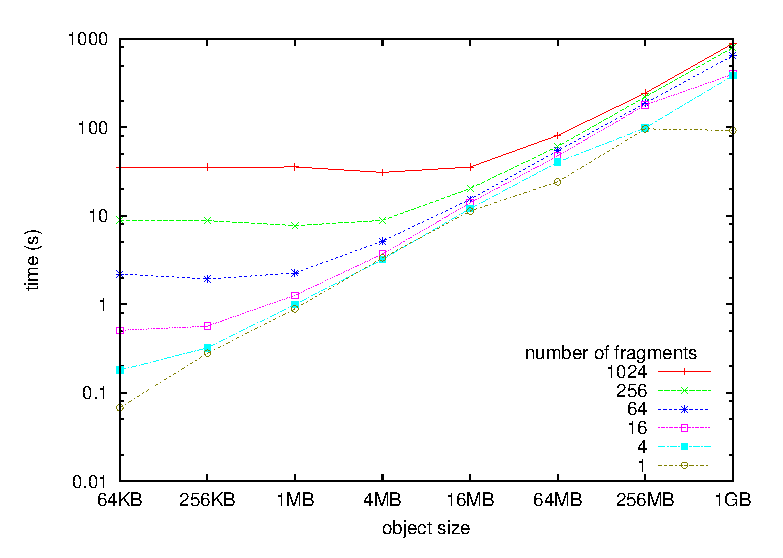
\includegraphics[width=0.8\columnwidth,valign=t]{figures/fig10}
\caption{\label{ms:fig:getPlain}Time for the execution of {\tt get} requests on Swift}
\end{figure}

\subsubsection{Experiments on the Overlay solution}
We built a Swift client application in Python that implements the {\tt get} and {\tt put\_fragment} methods that characterize our technique. We followed two implementation strategies, one using fragments as atomic separate objects, and the other adopting the DLO support offered by Swift.

Figure~\ref{ms:fig:getPlain} compares, for different numbers of fragments, the time required for the execution of {\tt get} requests assuming to map each fragment to a separate object. The lines correspond to distinct values for the number \fnum\ of fragments (i.e., 1, 4, 16, 64, 256, and 1024). The parameters that drive the performance are the network bandwidth and the overhead imposed by the management of each request. For {\tt get} requests, the overhead introduced by the management of one request for each fragment dominates when the resource is small, whereas the increase in object size makes the network bandwidth the bottleneck. The profile of {\tt put} requests uploading the complete resource proved to be identical to the profile of {\tt get} requests using a single fragment. The execution of {\tt put\_fragment} requests grows linearly with the size of the fragment.

The identification of the best number of fragments requires to consider the profile of the scenario. We evaluated the behavior of a system on a collection of 1000 objects where, after each {\tt put\_fragment} request, a sequence of 50 {\tt get} requests were executed on objects in the collection, all of the same size. Figure~\ref{ms:fig:throughputMget} reports the results of these experiments. As objects become larger, the benefits of fragmentation in the application of policy updates compensate for the overhead imposed on the retrieval of the objects. It is noted that the performance of the solution that does not use our technique corresponds to the line with one fragment. The throughput of the configurations using fragments is orders of magnitude higher already for medium-size objects. The graph also shows that the best number of fragments depends on the resource size. The identification of the value to use requires to consider the configuration of the system and the expected workload.

\begin{figure}[t]
\centering
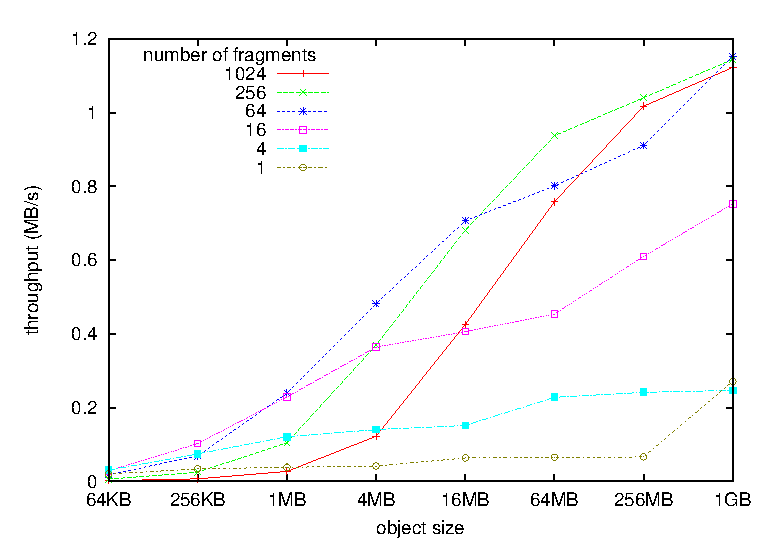
\includegraphics[width=0.8\columnwidth,valign=t]{figures/fig11}
\caption{\label{ms:fig:throughputMget}Throughput for a workload combining {\tt get} and {\tt put\_fragment} requests on Swift}
\end{figure}

A second set of experiments followed the same approach, but considering the use of DLOs in Swift. The number of fragments still has a significant impact on the performance of the {\tt get} request, because the server has to generate internally the mapping for the single request originating from the client and the multiple requests addressed to the storage nodes. The application of the same workload considered for the experiments in Figure~\ref{ms:fig:getPlain}, which interleaves {\tt get} and {\tt put\_fragment} requests, produces the results presented in Figure~\ref{ms:fig:throughputDlo}. Comparing the cost with and without DLO we notice a significant benefit deriving from the use of DLOs.

\subsection{Ad-hoc solution \label{ms:sec:adhoc}}
The use of an ad-hoc protocol is able to provide the full range of benefits of our approach. The protocol will have to support the basic primitives to upload ({\tt put}) and download ({\tt get}) a resource. The {\tt put} primitive, when used to upload the initial state of the resource, will have to provide a resource descriptor that defines: the identifier of the key \key{0} used by the owner to encrypt the resource; the size of mini-blocks and the number of fragments (which determine the size of the macro-block); an array with an element for every fragment describing its version. In addition to the {\tt put} primitive, the server will recognize the {\tt put\_fragment} primitive, which will allow the owner to update a fragment. Parameters of this primitive, in addition to the resource identifier and fragment content, will be the identifier of the fragment and its version number. The {\tt put\_fragment} primitive requires the authentication of the user issuing the request, in the same way as the {\tt put} primitive.

The {\tt get} primitive can return to the user the resource, one macro-block after the other. The client will be able to immediately start the decryption of macro-blocks, after a preliminary decryption with key \key{i} of the mini-blocks belonging to the fragments at version $i>0$. In this way, the client does not have to wait for the completion of the download of all the fragments. The answer to the {\tt get} request always provides first the resource descriptor, with the representation of the version of each of the fragments. Among the parameters of the {\tt get} primitive we have the option to retrieve only a specific portion of the resource.

For this solution, we have to dedicate attention to the mapping of the logical structure to the physical representation of data. At the logical level, the resource is divided into fragments, and the content is represented by a sequence of macro-blocks. At the physical level, the resource can be stored as a collection of separate fragments or as a sequence of macro-blocks. In addition to these two options, there is a range of intermediate alternatives, with the interleaved representation of multiple fragments.

\subsubsection{Experiments on the Ad-hoc solution}
The advantage of a dedicated server is the ability to use an efficient protocol. The use of an ad-hoc server makes the management of fragments more flexible and avoids the overheads associated with the generation of a number of independent {\tt get} requests equal to the number of fragments that are produced by the Overlay solution. Still, the use of a potentially large number of fragments can introduce non-negligible costs. In the extreme case where a large resource is managed with a single macro-block (i.e., the number of fragments corresponds to the number of mini-blocks of the whole resource), the client will have to wait for the download to complete to start decryption, and decryption will involve a high number of rounds. Also, when only a portion of the resource is needed, our approach requires the client to download the macro-blocks that contain the portion of interest; if macro-blocks are large, this may lead to a significant overhead. As already discussed, the identification of the optimal number of fragments has to consider several features of the application domain. In the current technological scenario, we notice that the use of an ad-hoc server can support a number of fragments larger than what is adequate for the Overlay solution, but extreme values cause inefficiencies.

\begin{figure}[t]
\centering
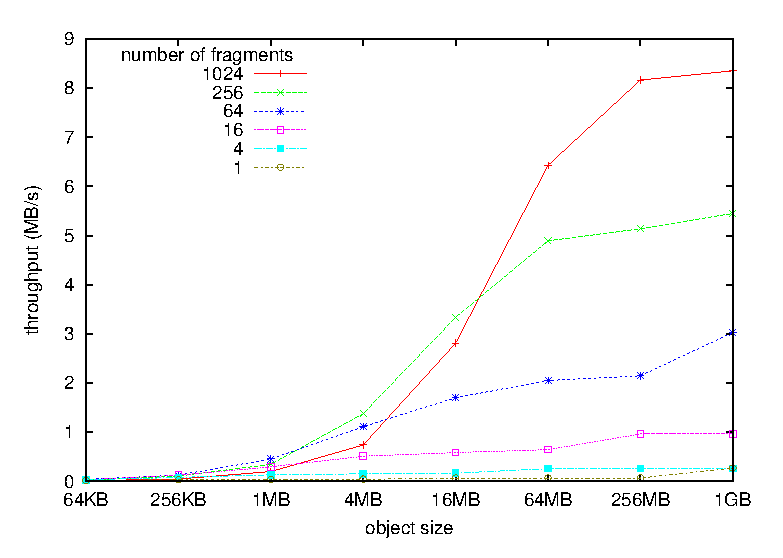
\includegraphics[width=0.8\columnwidth,valign=t]{figures/fig12}
\caption{\label{ms:fig:throughputDlo}Throughput for a workload combining {\tt get} and {\tt put\_fragment} requests with Swift DLOs}
\end{figure}

As mentioned above, an important aspect that the implementation of the ad-hoc server has to consider is the mapping from the logical structure to its physical representation. In this analysis, we will consider a traditional scenario where the server uses the functions of the operating system to access the storage ability of mass memory devices. In the experiments we used the Amazon EC2 instance and its access to the Elastic Block Storage. The operating system offers an interface that allows to read and write physical blocks, typically a few KiB in size. The mapping of the bidimensional logical structure with macro-blocks and fragments to the concrete physical structure realized by a sequence of physical blocks can follow several strategies. To compare these alternatives, we assume a scenario where we have 1024 fragments and map the structure to 4KiB physical blocks. A first strategy consists in storing the resource one macro-block after the other. The dual strategy consists in storing the resource one fragment after the other. Between these two extremes, we have strategies that split each macro-block into a number of parts and store contiguously into a physical disk block all the macro-block portions that correspond to the mini-blocks in the same position. The rationale is that the organization along macro-blocks will be the most efficient to support {\tt get} requests, but it will require to access all the physical disk blocks when a {\tt put\_fragment} request is received. The representation based on fragments will instead be the most efficient to support {\tt put\_fragment} requests, but it will introduce a significant overhead when managing {\tt get} requests. For small resources these aspects do not have a large impact, whereas for large resources the performance benefit can be significant. Figure~\ref{ms:fig:physical} illustrates the results obtained on a container with 1000 files, each of 1 GiB in size. The horizontal axis denotes the number of shares of each macro-block (1 represents the strategy with the macro-blocks stored in sequence, and 1024 represents the strategy with fragments stored in sequence). For a workload that interleaves a {\tt get} request for every {\tt put\_fragment} request, the total cost is minimized when we use a solution with 256 fragments. Interestingly, the two extremes with this workload do not represent the best option. In these experiments, we measured the time required to access the data from storage. In most systems we expect the network to be the bottleneck that limits the performance and the choice of physical representation will rarely be observed by the clients, but the performance benefit that is shown by the experiment can lead to a more efficient implementation of the server.

\begin{figure}[t]
\centering
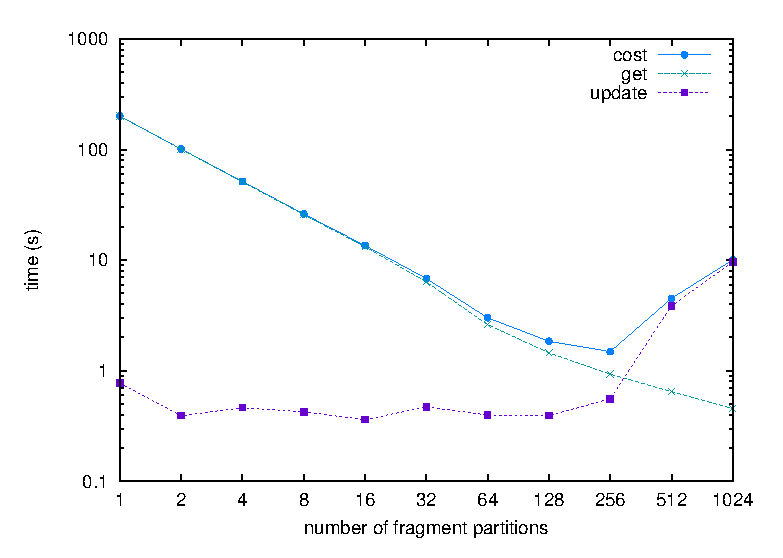
\includegraphics[width=0.8\columnwidth,valign=t]{figures/fig13}
\caption{\label{ms:fig:physical}Configurations for physical blocks}
\end{figure}
